\documentclass[tikz,convert={density=150,size=600,outext=.png}]{standalone}
\usetikzlibrary{shapes, calc, arrows, fit, positioning, decorations, patterns, decorations.pathreplacing, chains, snakes}
\input{../setup-web-fonts}
\input{../setup-packages}
\graphicspath{{../pictures/}} % path to pictures, trailing slash is mandatory.

\begin{document}
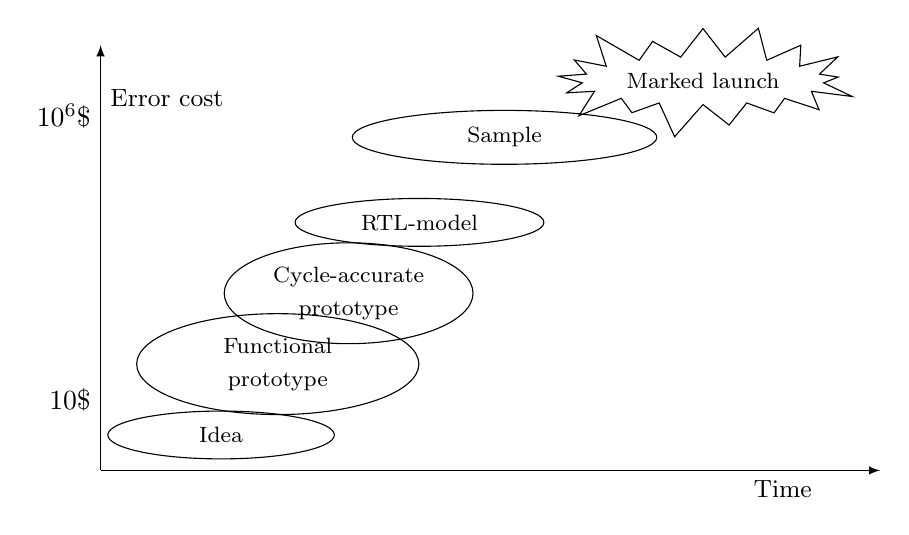
\begin{tikzpicture}[scale=0.9, >=latex]
    \draw[->] (0,0) -- (0,6)  node[very near end, right, text width = 3cm, text badly ragged] {\small{Error cost}};
    \draw[->] (0,0) -- (11,0) node[very near end, below] {\small Time};
    \path (0, 1) node[left] {$10 \$$};
    \path (0, 5) node[left] {$10^6 \$$};

    \path (1.7, 0.5) node[ellipse, draw, text width=1.8cm, text centered] {\footnotesize Idea};
    \path (2.5, 1.5) node[ellipse, draw, text width=2.3cm, text centered] {\footnotesize Functional prototype};
    \path (3.5, 2.5) node[ellipse, draw, text width=2cm, text centered] {\footnotesize Cycle-accurate prototype};
    \path (4.5, 3.5) node[ellipse, draw, text width=2cm, text centered] {\footnotesize  RTL-model};
    \path (5.7, 4.7) node[ellipse, draw, text width=2.5cm, text centered] {\footnotesize Sample};

    \path (8.5, 5.5) node[starburst, draw] {\footnotesize{Marked launch}};
\end{tikzpicture}
\end{document}
